\chapter{Splining}
\label{sec:splining}
Splining has been a popular approach in the community for optimizing the speed of lower-dimensional potentials\cite{todo}
The idea is to express a \"complex\" function piecewise with "less complex" spline functions.
One can think of as describing a higher-order function with a lot of lower-order functions.
The splining procedure can be split into two subproblems.
Given an input to evaluate the function we need to find the corresponding constrained domain and then evaluate the spline function.

There exist different approaches in splining techniques in atomistic learning.
\papercomment{
\begin{itemize}
  \item splining the radial part $R_{nl}$ or $R_{n}$ (Caro)
  \item splining potential in invariant space
\end{itemize}
}

\section{Grid}
The choice of grid determines

\subsection{Adaptive grid}

- O(log N) binary search lookup time but reduced error for same number of points (consider that a familiy of potenitals don't have any important information at the center
% talking abotut advai
%Optimization always can happen on multiple levels.
%On the level of optimizing the splining algorith, a very dynamic algorithm with adaptive domain size would be most optimal.
%Even when ignoring the time to actually compute such a the spline, by chosing the.
\subsection{Equispaced grid}
\begin{itemize}
\item O(1) constant lookup time but not optimal error
\item Uniform paralleization guarantees (not breaking out of for loop)
\end{itemize}

\section{Spline function}
- In principle tradeoff between higher-orders Easier fun
  But usually we do not have access to higher derivatives due to their complexity
- 

...
\subsection{Cubic spline}
\label{sec:cubic_spline}
As part my work in the first year, I participated in the development of a library designed to allow efficient computation of atomic density based descriptors, named librascal.
%The library is designed with most emphasize on efficiency with regard to code structure and computation methods of descriptors.
%The code structure is focused on reducing runtime cost by allowing a contiguous iteration through atomic environments and by applying template based methods as curiously recurring template pattern (CRTP) to prevent runtime lookups of virtual functions with the tradeoff of higher compile time costs.
My main contribution in the last year has been the development of efficient methods for the computation of the radial basis expansion for the SOAP descriptor.
In contrast to the approaches discussed in Section~\ref{sec:evaluation_of_radial_contribution}, for librascal Gaussian typed orbital (GTO) functions are used as radial basis functions 
\begin{subequations}
\begin{align}
R_n^{GTO}(r) = r^{n+2}\exp(-b_nr^2)N_n,\hspace{5em}\\
\text{with } b_n = 1/(2\sigma_n),\quad \sigma_n = r_c\,\textrm{max}(\sqrt{n},1)/n_{\text{max}},
% Remark: I added the factor r^2 to the basis function to be comparable with other publications
\end{align}
\end{subequations}
%Performance test done with the descriptor library Dscribe show a speed up of $10.07\pm 0.56$ times of the GTO basis over the polynomial one\cite{himanen2020dscribe}.
%In librascal the GTO improve the expansion on the radial part is to separate the radial and angular part in the original atomic density function as proposed by Marco...
that allow computing analytically the integral for the radial expansion in Eq.~\ref{eq:radial_part_in_spherical_expansion}. 
However, due to the modified spherical Bessel function $i_l$ %in Eq.~\ref{eq:radial_part_in_spherical_expansion}
an analytical expansion of radial term requires the evaluation of the computationally expensive confluent hypergeometric function $\hyponefone$ 
\begin{multline}
    \label{eq:radial_integral}
    \int_0^{\infty} R_n^{GTO}(r) \exp[-a(r^2+r_{ij}^2)]i_l(2arr_{ij}) \,\mathrm{d}r
    %\langle rlm|\mathcal{X}_i\rangle_{\hat{R}\hat{t}}\,\mathrm{d}r
    = N_n \pi^{\frac32}\frac{\Gamma(\frac{n+l+3}{2})}{\Gamma(l+\frac32)} \\
    (a+b)^{-\frac{n+l+3}{2}} (ar_{ij})^l \exp[-ar_{ij}^2] \hyponefone\big(\frac{n+l+3}{2},l+\frac32,\frac{a^2r_{ij}^2}{a+b}\big) = f^{nl}(r_{ij}).
\end{multline}
The contribution of this function to the overall cost of the radial expansion can be seen in Fig.~\ref{fig:hyp1f1_contribution} ranging from 55\% to 75\%  of the total time.
The term in Eq.~\ref{eq:radial_integral} can be expressed as a one dimensional function $f^{nl}$ of the distance $r_{ij}$ only dependent on the radial and angular numbers $n$ and $l$.
The computation of this term can be bypassed by interpolating the function for each $l,n$ term on the grid $[0,r_c]$.
An implementation of cubic spline interpolation for the term has been part of my work for the first year.
A spline interpolation splits the targeted range $[0,r_c]$ into intervals, each interval being interpolated by a polynomial with same boundary conditions.
Let $\{r_k\}_{k=1}^{M+1}$ be the set of $M+1$ boundary points in the interval $[0,r_c]$, then cubic spline defines polynomials $p_k(r) = A_k + B_kr + C_kr^2 + D_kr^3$ on the interval $[0,1]$ with the boundary conditions
\begin{subequations}
%\label{eq:abscissas_boundary_conditions}
\begin{align} 
    p^{nl}_{k}(0) = f^{nl}(r_k)&\text{ and } p^{nl}_{k}(1) =  f^{nl}(r_{k+1})\text{ for } k=1,\ldots,M , \label{eq:function_boundary_conditions}\\
    p^{nl}_{k}(0) = p^{nl}_{k-1}(1)&\text{ and } p^{nl}_{k}\prime(0)= p^{nl}_{k-1}\prime(1) \text{ for } k=2,\ldots,M  ,\label{eq:points_boundary_conditions}\\
    p^{nl}_k(1) = p^{nl}_{k+1}(0)&\text{ and }  p^{nl}_k\prime(1) = p^{nl}_{k+1}\prime(0) \text{ for } k=1,\ldots,M-1 ,\label{eq:derivative_boundary_conditions}\\
    p^{nl}_{1}\prime\prime(0) = 0&\text{ and } p^{nl}_{M}\prime\prime(1) = 0.\label{eq:natural_boundary_conditions}
\end{align}
\end{subequations}
The boundary conditions ensure the smoothness at the boundary points.
A linear system of equations can be formed from the $4M$ conditions in Eqs.~\ref{eq:points_boundary_conditions},~\ref{eq:derivative_boundary_conditions},~\ref{eq:natural_boundary_conditions} and their evaluation in Eq.~\ref{eq:function_boundary_conditions} by rearranging them\cite{bartels1995introduction} resulting in
\begin{subequations}
\begin{align}
A_k = f(r_k),\quad C_k = 3(f^{nl}(r_{k+1})-f^{nl}(r_k)) - 2B_k-B_{k+1},\\
D_k = 2(f^{nl}(r_{k})-f^{nl}(r_{k+1})) + B_k+B_{k+1},\hspace{5em}\\
\begin{pmatrix}
    2 & 1       &           &       &    \\
    1 & 4       & 1         &           &    \\
      & \ddots  & \ddots    & \ddots    &           \\
      &         & 1         &     4     & 1   \\
      &         &           &     1     & 2
\end{pmatrix}
\begin{pmatrix}
B_1\\
B_2\\
\vdots\\
B_{M-1}\\
B_{M}
\end{pmatrix}
=
\begin{pmatrix}
3(f^{nl}(r_2)-f^{nl}(r_1))\\
3(f^{nl}(r_3)-f^{nl}(r_1))\\
\vdots\\
3(f^{nl}(r_M)-f^{nl}(r_{M-2}))\\
3(f^{nl}(r_M)-f^{nl}(r_{M-1}))
\end{pmatrix}.
\end{align}
\end{subequations}
A linear systems forming a tridiagonal matrix can be solved in linear time with time complexity $O(2M)$ by iterating two times through the matrix following a Gaussian elimination scheme.
%\begin{equation}
%    
%\end{equation}
%In the forward pass the lower off diagonal is eliminated to zero, in the backward path the upper path is eliminated to zero.

Commonly, for interpolators the grid size is adaptively changed until it is below an error bound given by the user as input.
The error can be estimated by sampling points in the intervals $[r_k,r_{k+1}]$ and comparing the results of $f^{nl}$ with $p^{nl}$.
During implementation it has been shown that conditioning the error on a relative and absolute error has been most robust in terms of interpolation accuracy and convergence of the grid size.
This means that the boundary points are extended until one of the two estimated errors lies under the given error.

A point $r$ can be evaluated by first searching the corresponding boundary point $r_k$ for which $r\in[r_k,r_{k+1}]$, and then mapping $[r_k,r_{k+1}]$ to the polynomial interval $[0,1]$ with $p_k((r-r_k)/(r_{k+1}-r_k))$.
The design choice mainly affecting the efficiency of the cubic spline interpolator was the choice of the grid.
For an arbitrary grid with $M+1$ points, the optimal complexity for searching the boundary point $r_k$ is $O(\log(M+1))$ with a binary search.
On the other hand for uniform grids the search time can be reduced to $O(1)$ by
\begin{equation}
    k = \min(M,\lfloor (r-r_1)\Delta \rfloor+1), \quad \Delta = (M+1)/(r_{M+1}-r_1).
\end{equation}
%A non-uniform grid can keep the size of the grid to a minimum by only adding boundary points corresponding to the intervals with the highest error.
%This minimizes the number of evaluations of the costly function $f^{nl}$.
%With increasing number of evaluations of the function $f^{nl}$ the uniform grid will be always the better choice.
%Even though for realistic datasets with a limited number of evaluations this overhead could be crucial, it has been shown during implementation that the space overhead of a uniform grid is insignificant in comparison to the higher time complexity of the non-uniform grid.
\begin{figure}
    \centering
    \includegraphics[width=0.5\textwidth]{fig/fig_hyp1f1_contribution_in_radial_contribution.pdf}
    \caption{}
    \label{fig:hyp1f1_contribution}
\end{figure}
\begin{figure}
    \includegraphics[width=\textwidth]{fig/slide20_2.png}
    \caption{Effect of accuracy on prediction error}
    \label{fig:spline-accuracy-prediction-error}
\end{figure}\\
\begin{figure}
    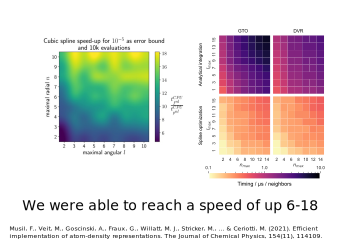
\includegraphics[width=\textwidth]{fig/slide20_3.png}
    \caption{Speedups}
    \label{fig:spline-speedups}
\end{figure}
%\caption{Distinct benchmarks with Intel i7-4770@3.4GHz for performance analysis of the evaluation of the radial term in Eq.~\ref{eq:radial_integral} and the speed-ups of cubic spline.}

For each $(n,l)$ pair a cubic spline interpolator is computed.
The effect of the speed-up for a reasonable range of $(n,l)$ pairs for $10k$ evaluations ranges from 6 up to 18 times as seen in Fig.~\ref{fig:cubic_speed_up}.
The exact speed up depends on the exact error bound as seen in Fig~\ref{fig:simd_comparison}.
By using the same grid for each $(n,l)$ pair, the matrix solver for tridiagonal matrices and the interpolation of a point $r$ for all $(n,l)$ can be vectorized.
Vectorization allows the parallel execution of the same instruction on multiple $(n,l)$ pairs.
These instructions are commonly known as single instruction, multiple data (SIMD) and their exact effect on the efficiency depend on the supported instruction set of the CPU architecture and the compiler.
The exact effect of the SIMD instructions for the implemented vectorized operations is a tedious task, since other parts of the code also rely on SIMD instructions\cite{mathuriya2017optimization}.
Therefore we limit our analysis to the effect of the SIMD optimization induced by the linear algebra library Eigen\cite{guennebaud2014eigen} used for the vectorized operations.
The optimization can be deactivated with the compiler option EIGEN\_DONT\_VECTORIZE.
A deactivation did not effect the performance significantly as seen in Fig.~\ref{fig:simd_comparison}.
A more exact analysis of the effect of the vectorization as in Ref.~\cite{mathuriya2017optimization} is part of future work.

In summary, due to the polynomial evaluation of cubic spline on a equispaced grid we gain speed-ups for the evaluation of the radial contribution ranging from 5.5 to 18 for commonly used radial and angular numbers.

\papercomment{
Boundary conditions: Three boundary conditions for Cubic spline, check with Hermite
- natural boundary
}

%\subsection{Hermite cubic spline [optional]}

%\section{Future directions - Splining spherical expansion}
%For a lot of ML model styles the spherical expansion coeffs are still essential 
%\papercomment{
%\begin{itemize}
%\item speed up
%\item potentially more numerical stability using different procedures to compute spherical harmonics, analytical evalutuion of 1F1 has problems for small sigma and large cutoff (double check)
%\end{itemize}
%}
%
%\subsection{Cache friendly design for splining atomistic data}

% lookup code of UF
%\begin{lstlisting}
%int start_index;
%if (knot_vect.front() <= r && r < knot_vect.back()) {
%  //Determine the interval for value_rij
%  for (int i = 3; i < knot_vect_size - 1; ++i) {
%    if (knot_vect[i] <= r && r < knot_vect[i + 1]) {
%      start_index = i;
%      break;
%    }
%  }
%}
%
%\end{lstlisting}
% TODO cite if needed
% https://github.com/uf3/uf3/blob/ab3003d128323295d1053562334c77ef807424c3/lammps_plugin/ML-UF3/uf3_pair_bspline.cpp#L59-L68}

%Improvements NL:
%\begin{itemize}
%  \item avoid recomputation of strict NL (but updating distances) by using skin of LAMMPS to reduce wrong branch prediction (in LAMMPS one can use skin)
%\end{itemize}
%Improvements Splining
%\begin{itemize} 
%  \item \textbf{Algorithmic:} constant time lookup by chosing regular grid (I don't know the reason why UF doesn't do it)
%  \item \textbf{Parallelism:} multithreading different hardware architectures support (by using Kokkos user package)
%  \item \textbf{Accuracy:} higher body order, as 3-body might be not enough but 4-body is competetive with nonlinear kernel methods, but since we are splining directly the higher-body function, we don't need to go directly to 4-body, we can do something like a 3.5-body order
%  \item \textbf{Cache locality:} sequential access of coefficients by sorting the grid as the access of the neighborlist (avoids random accesses https://www.quora.com/Is-sequential-access-to-RAM-faster-than-random) 
%  \item \textbf{Cache locality:} cmaybe SOA style iteration over grid points to take advantage of full cache lining and reduce thread numbers (instead of iterating over each grid point to compute like 6 coeffs, we iterate over the first coeff for all grid points)
%  %\item \textbf{Branch prediction:} theoretical some branches can be made more optimal (e.g. there is an if-case in compute for if UF3 is used), but most likely branch prediction optimizes it away
%  User interface
%  %\item \textbf{Branch prediction:} better initial guess for maxshort (size of triplet neighborlist) for initial steps, but should not matter for average one
%\end{itemize}
%\section{Splining the three-body}
